\subsection{Response function}

\begin{frame}{Response function from deconvolution}

  \begin{figure}
    \centering
    \tikz[baseline]{
      \node[anchor=south] (i1) {\includegraphics[width=.5\linewidth]{noresm/noresm_raw_dark.pdf}};
    }
  \end{figure}

  \vspace{-6mm}
  \begin{center}
    % {\color{MainBlue!35}\textsc{deconvolution}}
    {\pgfsetfillopacity{0.35}
      \textsc{deconvolution}
    }
    \pgfsetfillopacity{1}
  \end{center}\vspace{-6mm}

  \begin{figure}
    \centering
    \tikz[baseline]{
      \node[anchor=south] (o1) {\includegraphics[width=\linewidth]{response_func_noresm1_choose_dark.pdf}};
    }
  \end{figure}

  \begin{tikzpicture}[overlay]
    \path[->,white] (5.3,6) edge (5.3,5.3);
  \end{tikzpicture}

  \note{
  \begin{itemize}
    \item The solid green line is the result of deconvolution using the NorESM
      dataset, with monthly resolution
    \item The response function is sampled only at whole years, starting
      at \(0, 1, 2, \ldots\)
    \item We re-sample to yearly resolution since the proxy data we want to
      test against have resolution down to one year
  \end{itemize}
  }

\end{frame}

\begin{frame}{Response function from deconvolution}

  \begin{figure}
    \centering
    \tikz[baseline]{
      \node[anchor=south] (i1) {\includegraphics[width=.5\linewidth]{response_func_noresm1_choose_dark.pdf}};
    }
  \end{figure}

  \vspace{-6mm}
  \begin{center}
    % {\color{MainBlue!35}\textsc{deconvolution}}
    {\pgfsetfillopacity{0.35}
      \textsc{convolution}
    }
    \pgfsetfillopacity{1}
  \end{center}\vspace{-6mm}

  \begin{figure}
    \centering
    \tikz[baseline]{
      \node[anchor=south] (o1) {\includegraphics[width=\linewidth]{noresm_raw_with_est_dark.pdf}};
    }
  \end{figure}

  \begin{tikzpicture}[overlay]
    \path[->,white] (5.3,6) edge (5.3,5.3);
  \end{tikzpicture}

  \note{
  \begin{itemize}
    \item The solid green line is the result of deconvolution using the NorESM
      dataset, with monthly resolution
    \item The response function is sampled only at whole years, starting
      at \(0, 1, 2, \ldots\)
    \item We re-sample to yearly resolution since the proxy data we want to
      test against have resolution down to one year
  \end{itemize}
  }

\end{frame}

\subsection{Temperature estimates}

\begin{frame}{Temperature of last two millennia}

  \begin{figure}
    \centering%
    \includegraphics[width=\linewidth]{estimate_historic/best_fit_raw_temp1_alone_dark.pdf}%
  \end{figure}

  \note{
  \begin{itemize}
    \item We now look at how well the response function recreates historic
      temperature
    \item The lines are reconstructed temperature and forcing data sets from
      the last two millennia, with temperature in red and forcing in blue (note
      the scale is different by a factor ten)
    \item The response function we obtained is convolved with the blue forcing
      signal, and give an estimated temperature shown as the yellow line
    \item Estimated temperature largely capture the temperature from the forcing
  \end{itemize}
  }

\end{frame}

\begin{frame}{Temperature of \(4\times\ce{CO2}\) experiment}

  \begin{figure}
    \centering
    \includegraphics<1>[width=\linewidth]{estimate_historic/temp_abrupt1_alone_dark.pdf}%
  \end{figure}

  \note{
  \begin{itemize}
    \item Taking a look back at the climate sensitivity, we now convolve the
      response function with a constant forcing representing a quadrupling of
      \ce{CO2} concentration from pre-industrial levels
    \item This is a common experiment to do to decide equilibrium climate
      sensitivity, where the temperature at two different equilibria is
      compared
    \item Able to capture the shape of a NorESM \(4\times\ce{CO2}\) experiment
  \end{itemize}
  }

\end{frame}
